\documentclass[11pt]{article}

\usepackage[margin=1in]{geometry}
\usepackage{booktabs}
\usepackage{graphicx}
\usepackage{amsmath}
\usepackage{xeCJK}
\usepackage{microtype}
\usepackage{hyperref}
\usepackage{float}

\setCJKmainfont{SimSun}
\setmainfont{Times New Roman}

\title{真实焦栈焦度曲线形态分型报告}
\author{SRTP Optical Mechanism Analysis}
\date{2026-06-22}

\begin{document}
\maketitle

\section{Research Question}

前几轮分析已经显示，真实焦栈中的 DFF 不稳定性不能由小幅全局层间平移单独解释，并且 low-margin、focus entropy、peak strength 等无参考指标能够定位局部 peak-layer 跳变。本轮进一步追问一个更接近论文方法论的问题：真实域的不可靠焦度响应是否具有可分解的形态结构。如果这些形态能够被识别，Simulation-to-Real 的重点就可以从单纯合成表面高度，扩展到合成真实焦栈中出现的焦度曲线分布。

\section{Method}

本报告读取真实焦栈目录中的 7 组样本，跳过层数不足 8 的目录。每组样本先缩放到最长边不超过 640 像素，再用 Laplacian focus measure 计算逐像素 focus volume。对每个像素提取 DFF peak layer、top-2 peak separation、focus margin、focus entropy、peak strength、saturation persistence、bright persistence、mean intensity 以及局部 peak-layer spike proxy。

在无真实高度标签的条件下，本轮不直接声明高度误差，而是构造 6 类无标注诊断形态：
\begin{enumerate}
  \item \texttt{confident\_single\_peak}: 清晰单峰响应；
  \item \texttt{flat\_ambiguous}: 低峰值间隔或宽平焦度响应；
  \item \texttt{multi\_peak}: top-2 峰值位于相距较远的层；
  \item \texttt{local\_peak\_spike}: DFF peak layer 与局部邻域不一致；
  \item \texttt{saturated\_highlight}: 多层持续高亮或饱和；
  \item \texttt{dark\_low\_signal}: 暗弱信号且峰值响应不足。
\end{enumerate}

\section{Samples}

\begin{table}[H]
\centering
\small
\begin{tabular}{ll}
\toprule
ID & Stack \\
\midrule
S1 & 1124 \\
S2 & 3D层纹 \\
S3 & 3D表面 \\
S4 & 圆孔50um \\
S5 & 磕碰孔5um \\
S6 & 钥匙尖头50um \\
S7 & 钥匙纹路100um \\
\bottomrule
\end{tabular}
\caption{Analyzed real focus-stack samples.}
\end{table}

\section{Aggregate Results}

\begin{table}[H]
\centering
\small
\begin{tabular}{lrrrr}
\toprule
Class & Mean fraction & Median fraction & Max fraction & Present stacks \\
\midrule
\texttt{confident\_single\_peak} & 49.5\% & 50.2\% & 53.8\% & 7/7 \\
\texttt{flat\_ambiguous} & 25.5\% & 22.9\% & 37.3\% & 7/7 \\
\texttt{multi\_peak} & 4.2\% & 5.0\% & 7.8\% & 6/7 \\
\texttt{local\_peak\_spike} & 3.8\% & 4.2\% & 4.3\% & 7/7 \\
\texttt{saturated\_highlight} & 1.8\% & 0.2\% & 6.5\% & 3/7 \\
\texttt{dark\_low\_signal} & 15.2\% & 15.6\% & 18.0\% & 7/7 \\
\bottomrule
\end{tabular}
\caption{Aggregate focus-curve morphology fractions over seven real stacks.}
\end{table}

\begin{figure}[H]
\centering
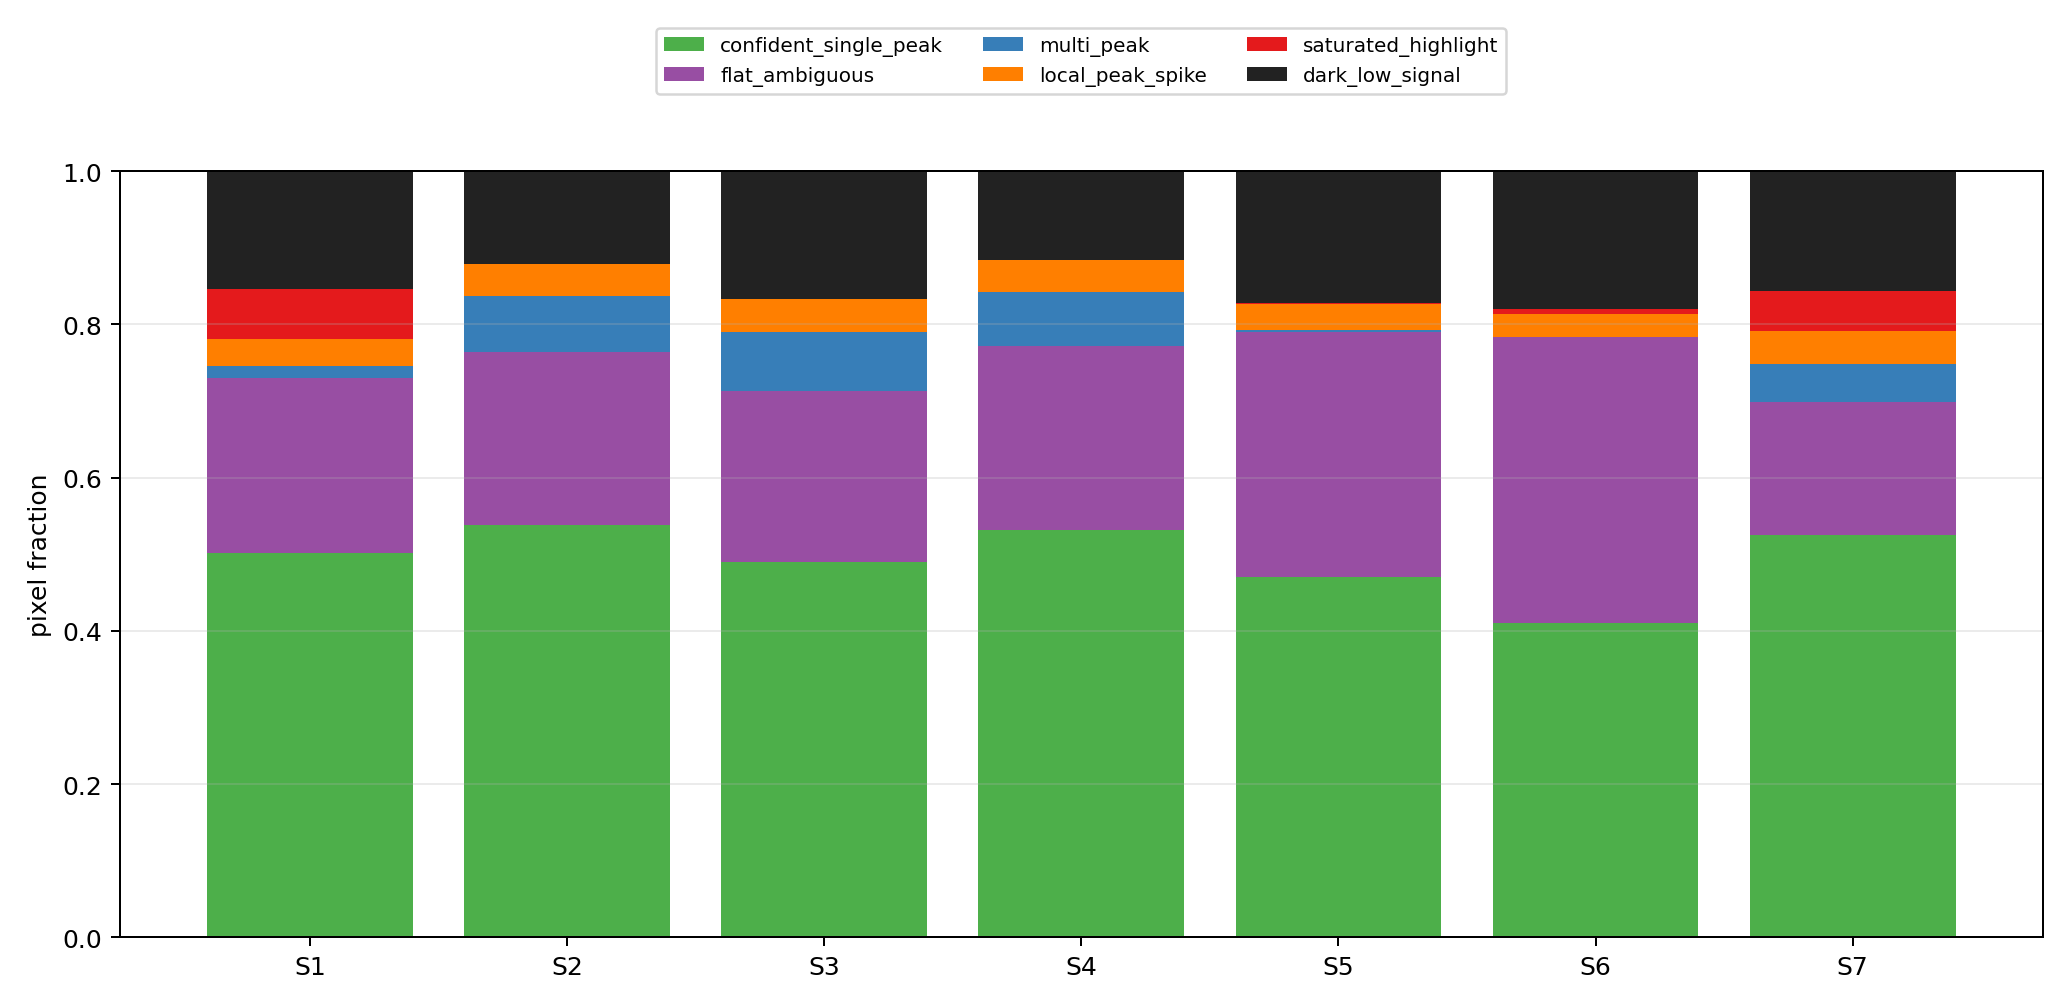
\includegraphics[width=\linewidth]{real_focus_curve_morphology/real_focus_curve_morphology_fractions.png}
\caption{Per-stack fractions of six focus-curve morphology classes.}
\end{figure}

\section{Representative Observation}

\begin{figure}[H]
\centering
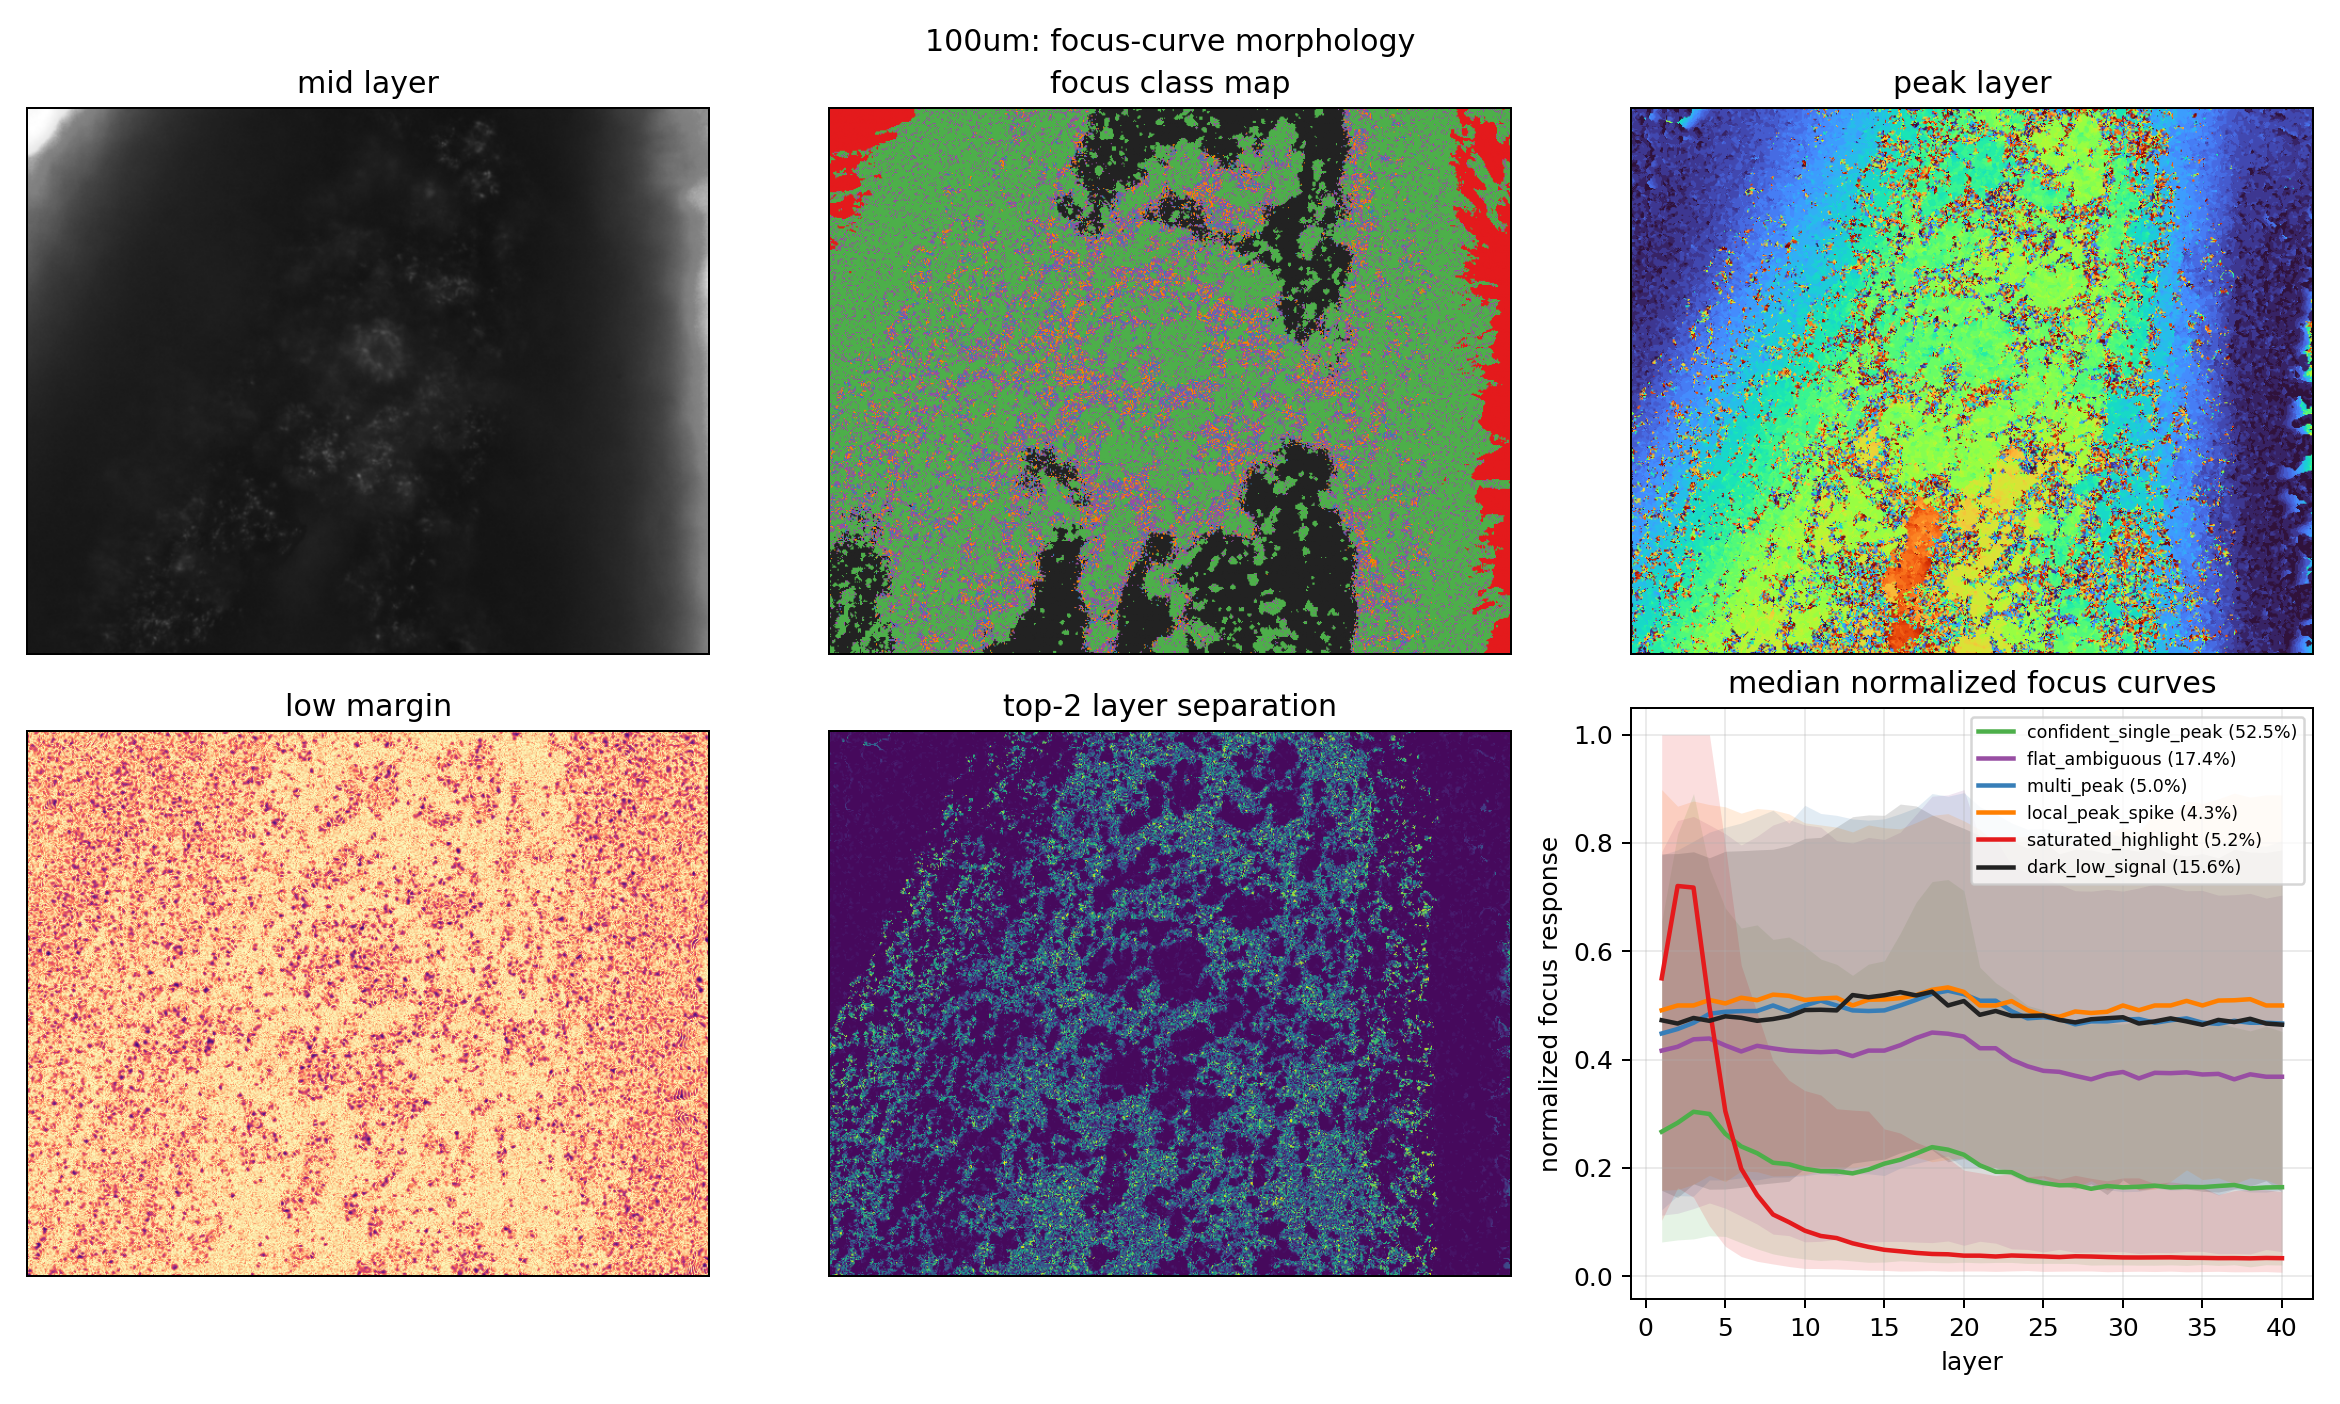
\includegraphics[width=\linewidth]{real_focus_curve_morphology/钥匙纹路100um_focus_curve_morphology.png}
\caption{Representative focus-curve morphology result on the S7 key-texture stack.}
\end{figure}

在 S7 样本中，\texttt{saturated\_highlight} 主要集中在右侧持续高亮边缘，并呈现早层强响应；\texttt{dark\_low\_signal} 分布在暗弱区域；\texttt{multi\_peak} 与 \texttt{local\_peak\_spike} 则更多对应纹理区域中的竞争峰值和局部层选择跳变。这说明同一真实焦栈内同时存在光照/饱和型异常、低信号型异常和焦度曲线竞争型异常。

\section{Interpretation}

7 组真实焦栈中，清晰单峰区域平均占 49.5\%，其余像素被分配到多类不可靠或弱约束形态。最主要的不确定来源是 \texttt{flat\_ambiguous}，平均占 25.5\%，说明真实焦栈中有大量像素的焦度曲线缺乏唯一峰值。暗弱信号平均占 15.2\%，局部 peak-layer spike 平均占 3.8\%，多峰竞争平均占 4.2\%。持续高亮饱和只出现在部分样本，平均占 1.8\%，但在最高样本中可达 6.5\%。

这组结果支持一个更细的论文主线：DFF 先验本身是有价值的，但它在真实域中应作为带置信度的观测来使用。模型训练阶段可以把焦度曲线形态作为三类信号引入：第一类是可靠单峰区域，用于强化几何监督；第二类是平坦、多峰、局部跳变区域，用于降低伪标签权重或训练 confidence head；第三类是高亮饱和和暗弱信号区域，用于指导仿真样本构造和 domain randomization。

\section{Simulation-to-Real Implication}

对 Simulation-to-Real 故事而言，本轮结果给出一个可执行的仿真目标：仿真器需要复现的不只是表面高度分布，还包括真实焦栈中的焦度曲线形态分布。具体而言，后续合成数据可以显式加入单峰清晰样本、低 margin 平坦样本、跨层多峰样本、局部 peak-layer 跳变样本、持续高亮饱和样本和暗弱信号样本。这样构造出的训练集更接近真实采集过程中的观测退化，而模型也可以通过样本权重、置信度分支或不确定性损失学习何时相信 DFF 先验。

\section{Paper-Ready Statement}

CN: 我们进一步对 7 组真实焦栈进行逐像素焦度曲线形态分型。结果显示，真实域中约 49.5\% 的像素呈现清晰单峰响应，其余区域主要由低峰值间隔的平坦响应、暗弱信号、跨层多峰竞争、局部 peak-layer 跳变以及持续高亮饱和构成。这表明 DFF 先验在真实域中更适合作为带置信度的观测，而不宜被视为处处可靠的监督标签。该发现也为 Simulation-to-Real 数据构造提供了更具体的目标：仿真过程应同时覆盖表面高度、焦度曲线形态和光照/饱和退化。

EN: We further conduct a per-pixel focus-curve morphology analysis on seven real focus stacks. On average, 49.5\% of pixels exhibit confident single-peak responses, while the remaining regions are distributed among flat low-margin responses, dark low-signal areas, separated multi-peak competition, local peak-layer spikes, and persistent saturated highlights. These results suggest that DFF priors in real domains should be treated as confidence-aware observations rather than uniformly reliable supervision. They also provide a concrete target for Simulation-to-Real data construction: synthetic stacks should cover not only surface height variations, but also focus-curve morphology and illumination/saturation degradations.

\section{Limitations}

该分型是无参考诊断，不替代真实高度误差评估。阈值按每组焦栈自适应设定，因此当前结果适合支撑机制分析、仿真设计和训练策略，而最终定量性能结论仍需要真实高度标签、重复采集或人工标注 ROI 进一步验证。

\end{document}
